%% Copernicus Publications Manuscript Preparation Template for LaTeX Submissions
%% ---------------------------------
%% This template should be used for copernicus.cls
%% The class file and some style files are bundled in the Copernicus Latex Package which can be downloaded from the different journal webpages.
%% For further assistance please contact the Copernicus Publications at: publications@copernicus.org
%% http://publications.copernicus.org


%% Please use the following documentclass and Journal Abbreviations for Discussion Papers and Final Revised Papers.


%% 2-Column Papers and Discussion Papers
%\documentclass[hess, manuscript]{copernicus}
\documentclass[hess]{copernicus}



%% Journal Abbreviations (Please use the same for Discussion Papers and Final Revised Papers)

% Archives Animal Breeding (aab)
% Atmospheric Chemistry and Physics (acp)
% Advances in Geosciences (adgeo)
% Advances in Statistical Climatology, Meteorology and Oceanography (ascmo)
% Annales Geophysicae (angeo)
% ASTRA Proceedings (ap)
% Atmospheric Measurement Techniques (amt)
% Advances in Radio Science (ars)
% Advances in Science and Research (asr)
% Biogeosciences (bg)
% Climate of the Past (cp)
% Drinking Water Engineering and Science (dwes)
% Earth System Dynamics (esd)
% Earth Surface Dynamics (esurf)
% Earth System Science Data (essd)
% Fossil Record (fr)
% Geographica Helvetica (gh)
% Geoscientific Instrumentation, Methods and Data Systems (gi)
% Geoscientific Model Development (gmd)
% Geothermal Energy Science (gtes)
% Hydrology and Earth System Sciences (hess)
% History of Geo- and Space Sciences (hgss)
% Journal of Sensors and Sensor Systems (jsss)
% Mechanical Sciences (ms)
% Natural Hazards and Earth System Sciences (nhess)
% Nonlinear Processes in Geophysics (npg)
% Ocean Science (os)
% Proceedings of the International Association of Hydrological Sciences (piahs)
% Primate Biology (pb)
% Scientific Drilling (sd)
% SOIL (soil)
% Solid Earth (se)
% The Cryosphere (tc)
% Web Ecology (we)



%% \usepackage commands included in the copernicus.cls:
%\usepackage[german, english]{babel}
%\usepackage{tabularx}
%\usepackage{cancel}
%\usepackage{multirow}
%\usepackage{supertabular}
%\usepackage{algorithmic}
%\usepackage{algorithm}
%\usepackage{amsthm}
%\usepackage{float}
%\usepackage{subfig}
%\usepackage{rotating}

\usepackage[utf8]{inputenc}


\begin{document}

\linenumbers

\title{The Analogue Method for Precipitation Forecasting: Finding Better Analogue Situations at a Sub-Daily Time Step}


% \Author[affil]{given_name}{surname}

\Author[1,2]{Pascal}{Horton}
\Author[3]{Charles}{Obled}
\Author[1]{Michel}{Jaboyedoff}

\affil[1]{University of Lausanne, Lausanne, Switzerland}
\affil[2]{Terranum, Lausanne, Switzerland}
\affil[3]{Universit\'{e} de Grenoble-Alpes, LTHE, Grenoble, France}

%% The [] brackets identify the author with the corresponding affiliation. 1, 2, 3, etc. should be inserted.



\runningtitle{Finding Better Analogue Situations at a Sub-Daily Time Step}

\runningauthor{P. Horton et al.}

\correspondence{Pascal Horton (pascal.horton@alumnil.unil.ch)}



\received{}
\pubdiscuss{} %% only important for two-stage journals
\revised{}
\accepted{}
\published{}

%% These dates will be inserted by Copernicus Publications during the typesetting process.


\firstpage{1}

\maketitle



\begin{abstract}
TEXT
\end{abstract}



\introduction  %% \introduction[modified heading if necessary]





%REWRITE

Multiple variations of the methods exist, and most of them will not be detailed hereafter \cite[see][for more comprehensive listings]{Horton2016, BenDaoud2015}. However, there are mainly 2 parameterizations that are most often used for precipitation forecasting and that will be considered as reference: one that relies on an analogy of the atmospheric circulation, and another that adds a second level of analogy on moisture variables \citep{Obled2002, Bontron2005, Marty2012}.

The method based on the analogy of the synoptic circulation consists in the following steps (Table \ref{table:method_2Z}): the similarity of the atmospheric circulation of a target date with every day of the archive is assessed by processing the S1 criteria \citep[Eq.\ \ref{eq:S1}, ][]{Teweles1954, Drosdowsky2003}, which is a comparison of gradients, over a certain spatial window. \citet{Bontron2005} showed that the geopotential height at 500~hPa (Z500) and 1000~hPa (Z1000) are the best first predictors of the NCEP/NCAR reanalysis dataset, and that the S1 criteria performs better than scores based on absolute distances. The reason for such better results is that the S1 criteria allows comparing the circulation pattern, by means of the gradients, rather than the absolute value of the geopotential height. To cope with seasonal effects, candidate dates are extracted within a period of 4 months centered around the target date, for every year of the archive. Following the nomenclature proposed by \citet{Horton2016}, this method will be named 2Z.

\begin{equation}
\label{eq:S1}
S1=100 \frac {\displaystyle \sum_{i} \vert \Delta\hat{z}_{i} - \Delta z_{i} \vert}
{\displaystyle \sum_{i} max\left\lbrace \vert \Delta\hat{z}_{i} \vert , \vert \Delta z_{i} \vert \right\rbrace }
\end{equation}
where $\Delta \hat{z}_{i}$ is the forecast geopotential height difference between the \textit{i}th pair of adjacent points of the gridded data describing the target situation, and $\Delta z_{i}$ is the corresponding observed geopotential height difference in the candidate situation. The differences are processed separately in both directions. The smaller the S1 values, the more similar the pressure fields.

\begin{table}[htb]
	\caption{Parameters of the reference method on the atmospheric circulation (2Z). The first column is the level of analogy (0 for preselection), then comes the meteorological variable and its hour of observation (temporal window). The criteria used for the current level of analogy is then provided, as well as the number of analogues.}
	\footnotesize
	\begin{center}
		\begin{tabular}{ccccc}
			\hline
			Level & Variable & Hour & Criteria & Nb \\ 
			\hline 
			0 & \multicolumn{4}{l}{$\pm 60$ days around the target date} \\
			\hline 
			\multirow{2}{*}{1} & Z1000 & 12~h & \multirow{2}{*}{S1} & \multirow{2}{*}{50} \\
			& Z500 & 24~h & & \\ 
			\hline 
		\end{tabular} 
	\end{center}
	\label{table:method_2Z}
\end{table}

The $N_{1}$ dates with the lowest values of S1 are considered as analogues to the target day. The number of analogues, $N_{1}$, is a parameter to calibrate. Then, the daily observed precipitation amount of the $N_{1}$ resulting dates provide the empirical conditional distribution considered as the probabilistic forecast for the target day.

The other most know parametrization adds a second level of analogy on moisture variables (method 2Z-2MI, Table \ref{table:method_2Z-2MI}). The predictor that \citet{Bontron2004} found optimal for the France territory is a moisture index made of the product of the precipitable water with the relative humidity at 850~hPa (RH850). \cite{Horton2012a} confirmed that this index is also better for the Swiss Alps than any other variable from the NCEP/NCAR reanalysis considered independently. When adding a second level of analogy, $N_{2}$ dates are subsampled in the $N_{1}$ analogues on the atmospheric circulation, to end up with a smaller number of analogue situations. When a second level of analogy is added, a higher number of analogues is kept on the first level.

\begin{table}[htb]
	\caption{Parameters of the reference method with moisture variables (2Z-2MI). Same conventions as Table \ref{table:method_2Z}}
	\footnotesize
	\begin{center}
		\begin{tabular}{ccccc}
			\hline 
			Level & Variable & Hour & Criteria & Nb \\ 
			\hline 
			0 & \multicolumn{4}{l}{$\pm 60$ days around the target date} \\
			\hline 
			\multirow{2}{*}{1} & Z1000 & 12~h & \multirow{2}{*}{S1} & \multirow{2}{*}{70} \\
			& Z500 & 24~h & & \\ 
			\hline
			\multirow{2}{*}{2} & TPW * RH850 & 12~h & \multirow{2}{*}{RMSE} & \multirow{2}{*}{30} \\
			& TPW * RH850 & 24~h & & \\ 
			\hline 
		\end{tabular} 
	\end{center}
	\label{table:method_2Z-2MI}
\end{table}

%REWRITE




%COMPLETE



sliding time window (STW)



The analogue method (AM) is usually implemented with a daily time step, due to the availability of long precipitation archives that have no equivalent to a finer resolution. Therefore, the analogues situations are compared on the basis of a daily time step, by comparing predictors at fixed hours of the day, otherwise we would not know what precipitation values to assign to them. However, we can expect that the analogy of the synoptic situations do not occur systematically at the same time of the day, and that better candidates can be found at different times.

Previous tests showed the benefit, in terms of analogy criteria values, of searching for analogue synoptic situations at a finer time step, but without assessing the impact on the forecast skills \citep{Finet2008}. Archives of sub-daily precipitation datasets were not available on a long period in order to assess the improvement of the prediction. In order to assess this potential gain, precipitation data with a resolution of 10 minutes on a respectable archive length was used (section \ref{sec:data}). It was then aggregated in the form of 24~h totals, but at a 6-hourly time step, by means of a moving average (section \ref{sec:method}).

One can question the interest of using daily totals when a 6-hourly precipitation series can be used. The first reason is that the 6-hourly time series generated by the AM may not represent well the dynamic of the accurate precipitation (results not shown), due to a smoothed signal. Then, sometimes we just don't need finer resolution than the daily time step. Finally, when using a reconstructed precipitation archive, the errors in intra-day precipitation distributions have a lesser impact.





%COMPLETE



\section{Study area and data}
\label{sec:data}

The study area is the upper Rh\^{o}ne catchment in Switzerland. Due to the low density of weather stations with high temporal resolution and long archives, no aggregation or catchment rainfall was processed. The time series (on the period 1982-2007) come from 6 automatic weather stations, namely Ulrichen, Zermatt, Visp, Montana, Sion and Aigle. The results will often be presented arbitrarily for the Ulrichen station, but the results are exactly the same for all stations.


%WRITE

%FIGURE


\section{Method}
\label{sec:method}

In order to assess the benefit of searching analogue situations at a sub-daily time step, an appropriate time series is required. On the basis of high resolution time series (section \ref{sec:data}), 24~h totals were processed, but at a 6-hourly time step (temporal resolution of the reanalysis dataset), by means of a moving average. 

The target situations and their corresponding observed precipitation values (used for validation) do not change, because the forecast is always established for a fixed period of the target day (6-30~h), as before. The difference is that the candidates are 4~times more numerous (Figure \ref{fig:principle}).

\begin{figure}[htb]
	\begin{center}
		
\includegraphics[width=8.3cm]{figures/illustration_moving_window.pdf}
	\end{center}
	\caption{Illustration of the principle of a sliding time window. }
	\label{fig:principle}
\end{figure}

Logic suggests a priori that only one situation (the best) is selected per candidate day. An exclusion of the same dates was tested in two different ways: (1)
by excluding the worse analogues in a period of $\pm$ 24~h, and (2) by excluding the worse analogues with the same date. After several tests, it turned out that no restrictions led to better skills, and this on a significant and recurring basis. Thus, no constraint was further used.


\section{Consequences of the archive reduction}

As sub-daily precipitation time series are usually available on a shorter period than traditional daily time steps, the first assessment consists in assessing the loss of performance resulting from a reduction a 47~years archive (1961 to 2008) to 25~years (1982 to 2007). This change is assessed with the original method, without STW.

Both 2Z (Table \ref{table:method_2Z}) and 2Z-2MI (Table \ref{table:method_2Z-2MI}) methods were considered. The AM parameters were calibrated on the original archive (Tables \ref{table:method_2Z} and \ref{table:method_2Z-2MI}) and will be used thereafter.

\begin{table}[htb]
	\caption{Calibrated parameters (spatial windows and number of analogues) for the analogy on the geopotential at 500~hPa and 1000~hPa (method 2Z) and skill score (\%) of the method on the full archive.}
	\begin{center}
		\begin{tabular}{l c c c c }
			\hline
			Station & Longitudes & Latitudes & N$_{1}$ & CRPSS \\
			\hline
			Ulrichen & 0 $\rightarrow$ 17.5 & 42.5 $\rightarrow$ 47.5 & 40 & 30.73 \\
			Zermatt & 0 $\rightarrow$ 20 & 37.5 $\rightarrow$ 50 & 35 & 23.87 \\
			Visp & -2.5 $\rightarrow$ 20 & 40 $\rightarrow$ 47.5 & 30 & 25.11 \\
			Montana & -2.5 $\rightarrow$ 17.5 & 40 $\rightarrow$ 47.5 & 40 & 32.55 \\
			Sion & -2.5 $\rightarrow$ 17.5 & 40 $\rightarrow$ 47.5 & 40 & 26.23 \\
			Aigle & -5 $\rightarrow$ 17.5 & 40 $\rightarrow$ 50 & 50 & 30.59 \\ 
			\hline
		\end{tabular}
	\end{center}
	\label{table:params_2Z}
\end{table}

\begin{table}[htb]
	\caption{Parameters of the moisture variables from the 2Z-2MI method and the corresponding skill score (\%) on the complete archive. The parameters for the atmospheric circulation are the same as in Table \ref{table:params_2Z}, except the number of analogues of the first analogy level (N$_{1}$), which are here different. The $5^{th}$ column is the number of analogues for the second level (N$_{2}$).}
	\begin{center}
		\begin{tabular}{l c c c c c }
			\hline
			Station & Longitudes & Latitudes & N$_{1}$ & N$_{2}$ & CRPSS \\
			\hline
			Ulrichen & 5 $\rightarrow$ 10 & 45 $\rightarrow$ 47.5 & 60 & 25 & 34.31 \\
			Zermatt & 5 $\rightarrow$ 10 & 45 $\rightarrow$ 47.5 & 55 & 25 & 28.28 \\
			Visp & 5 $\rightarrow$ 10 & 45 $\rightarrow$ 47.5 & 45 & 25 & 28.85 \\
			Montana & 5 $\rightarrow$ 7.5 & 45 $\rightarrow$ 47.5 & 55 & 30 & 36.11 \\
			Sion & 5 $\rightarrow$ 10 & 45 $\rightarrow$ 47.5 & 90 & 30 & 31.16 \\
			Aigle & 7.5 & 45 $\rightarrow$ 47.5 & 100 & 35 & 35.82 \\ 
			\hline
		\end{tabular}
	\end{center}
	\label{table:params_2Z-2MI}
\end{table}

\begin{table}[htb]
	\caption{Influence of the archive reduction on the CRPSS. CRPSS values are provided for both considered methods and the differences are expressed in absolute value.}
	\begin{center}
		\begin{tabular}{l c c c c }
			\hline
			\multirow{2}{*}{Station} & \multicolumn{2}{c}{2Z} & \multicolumn{2}{c}{2Z-2MI} \\
			& 82-07 & $\Delta$ & 82-07 & $\Delta$ \\ 
			\hline
			Ulrichen & 29.37 & -1.36 & 33.24 & -1.08 \\
			Zermatt & 22.20 & -1.67 & 26.95 & -1.32 \\
			Visp & 23.23 & -1.89 & 27.77 & -1.08 \\
			Montana & 30.79 & -1.76 & 34.77 & -1.34 \\
			Sion & 24.78 & -1.45 & 29.36 & -1.80 \\
			Aigle & 30.57 & -0.01 & 35.95 & 0.13 \\ 
			\hline
		\end{tabular}
	\end{center}
	\label{table:loss_reduction}
\end{table}

The impact of the change in the archive length is summarized in Table \ref{table:loss_reduction} for both 2Z and 2Z-2MI methods. As expected, a loss of performance can be observed for each station, except for that of Aigle, which seems relatively indifferent to this change. This loss is globally significant, with up to -1.89 points for Visp and the 2Z method. 


\section{Influence on the analogy criteria}

\subsection{Changes in the atmospheric circulation analogy}

When searching for analogues on the geopotential heights, as in the 2Z method, there are now 4 times more candidates than before, which obviously allows to find better matches.

\begin{figure*}[htb]
	\begin{center}
		\includegraphics[width=15cm]{figures/changes_S1_analogues.png}
	\end{center}
	\caption{Changes in the S1 criteria distributions of the $1^{st}$, $5^{th}$, $20^{th}$ and $40^{th}$ analogue ranks for the Ulrichen station, due to the STW.}
	\label{fig:changes_S1_analogues}
\end{figure*}

Figure \ref{fig:changes_S1_analogues} presents the changes in the distributions of the S1 criterion for the $1^{st}$, $5^{th}$, $20^{th}$ and $40^{th}$ analogues for the Ulrichen station on the whole calibration period, due to introduction of the STW. The precipitation target remains at before, that is centered on 18~h~UTC (6~h~UTC to 6~h~UTC the next day). The shapes of the distributions of the conventional approach and the STW are similar, but the values of the analogy criteria are now reduced, therefore better. An increase in the difference between a fixed window and a sliding window is identifiable, which means that the last analogues are further improved. The latter effect is due to the accumulation of improvements brought by the new analogue situations in the selection.

\begin{figure}[htb]
	\begin{center}
		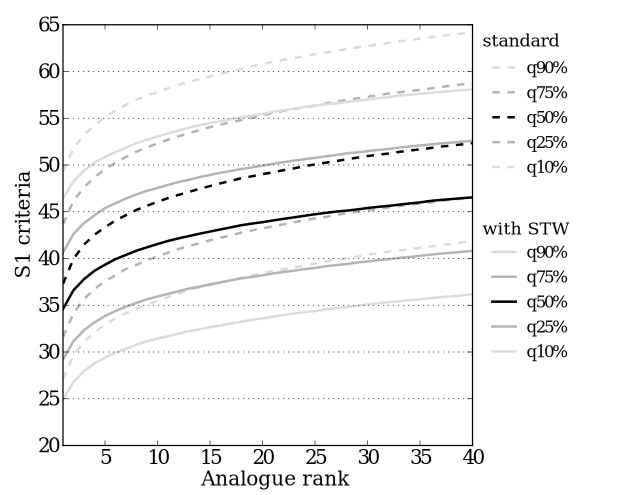
\includegraphics[width=8.2cm]{figures/changes_S1_value.pdf} \\
		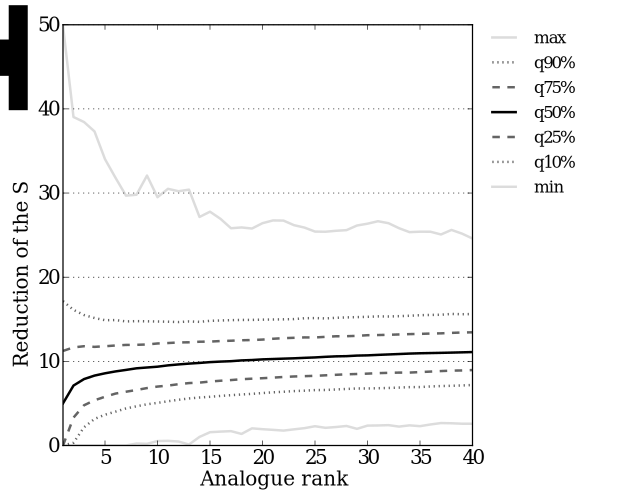
\includegraphics[width=8.3cm]{figures/changes_S1_gain.pdf}
	\end{center}
	\caption{Synthesis of the changes in the S1 criteria, due to the STW, for the Ulrichen station, depending on the ranks of the analogue. (top) Quantiles of the S1 distributions with and without the sliding window. (bottom) Quantiles of the relative improvements of the S1 criteria when using the sliding window.}
	\label{fig:changes_S1}
\end{figure}

The improvements of the S1 criteria are summarized in Figure \ref{fig:changes_S1}, which shows (top) quantiles of the S1 criteria according to the analogue rank for the conventional method and the STW, and (bottom) quantiles of the relative reduction. This confirms that all quantile seem similarly reduced (S1 distributions keep their shape), and that this improvement is constantly increasing from the first to the last analogue (Figure \ref{fig:changes_S1} bottom).

The median of the S1 values reduction (Figure \ref{fig:changes_S1} bottom) starts approximately at 5~\% for the first analogue and reaches more than 10~\% for the last. This increasing trend with the analogue rank can be explained by the accumulation of better analogues in the distribution. The minimum improvement starts from 0 and reaches 2-3\%, meaning that the criteria has been improved for all analogue ranks of the distribution end. All other stations have a similar improvement of the S1 criteria, both in terms of distribution shape and amplitude.


\subsection{Influence of the weather situation}
\label{sec:influence_precip}

It can be assumed that the atmospheric conditions with a low dynamism, such as the frequent anticyclonic situations, will not be radically improved by the introduction of the STW. Conversely, dynamic situations, such as weather disturbances, have a well marked temporal evolution. Indeed, the position of the driving elements such as the low-pressure area and the fronts change significantly during a day. We can therefore expect to improve particularly these situations with a higher dynamism when introducing a STW, as we may find better matches to the target situation.

The dynamism of a given atmospheric condition cannot be easily quantified. We thus consider here the basic assumption that the more a day is rainy, the more dynamic the situation is. The results of this analysis are summarized in Figure \ref{fig:changes_S1_precip_threshold} by the median reduction of S1 for days with precipitation between two thresholds. The number of analogues being reduced, the curves are not as smooth as in previous analyzes. It is nevertheless clear that the improvement tends to increase on days with higher precipitation. This is true for all our stations and confirms our intuition.

\begin{figure}[htb]
	\begin{center}
		\includegraphics[width=8.3cm]{figures/changes_S1_precip_threshold.pdf}
	\end{center}
	\caption{Distribution of the median improvements of the S1 criteria, due to the STW, depending on precipitation thresholds at the Ulrichen station.}
	\label{fig:changes_S1_precip_threshold}
\end{figure}


\subsection{Seasonal effect}
\label{sec:seasonal_effect}

Atmospheric dynamics varies greatly from one season to another, which reflects on the performance of the AM that is generally lower between June and August \citep{Bliefernicht2010}. It therefore makes sense to verify the effect of the STW separately per season.

\begin{figure}[htb]
	\begin{center}
		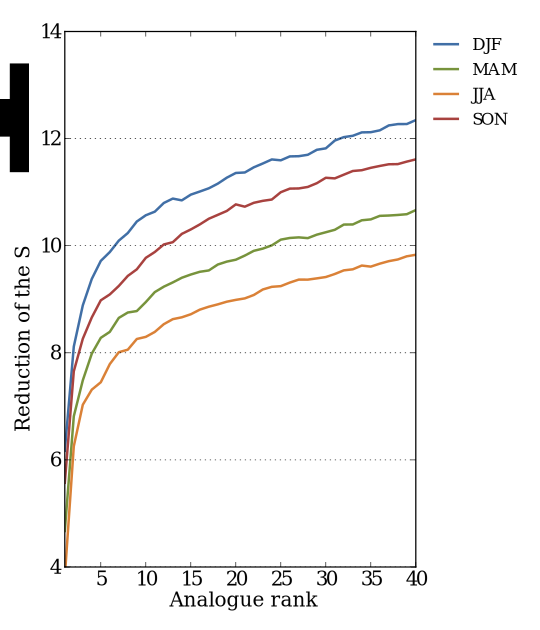
\includegraphics[width=7cm]{figures/changes_S1_seasons.pdf}
	\end{center}
	\caption{Seasonal effect on the median reduction of the S1 criteria for the Ulrichen station due to the sliding time window. DJF: winter, MAM: spring, JJA: summer SON: fall.}
	\label{fig:changes_S1_seasons}
\end{figure}

\begin{figure}[htb]
	\includegraphics[width=8.3cm]{figures/hours_selection_per_season.pdf}
	\caption{Distribution of the predictors hours in the selected analogue dates depending on the season, for the Ulrichen station.}
	\label{fig:hours_selection_per_season}
\end{figure}

A seasonal effect can be observed on the reduction of the S1 criteria due to the STW (Figure \ref{fig:changes_S1_seasons}). The improvements are greater for winter than summer. One hypothesis is that the diurnal effects of the summer months have an influence on the atmospheric circulation, at least in the lower layers. This effect is based on the daily cycle and good analogues for the same hours are already selected.

An analysis of the selected hours for the geopotential predictor seems to confirm this assumption (Figure \ref{fig:hours_selection_per_season}). It was found that the new choice of the temporal window in winter, when using the STW approach, is well balanced between the 4 options. This means a change of 75\% of the analogues selection compared to the conventional approach, which improves the circulation analogy.

On the contrary, the summer months have a preference for the initial temporal window (Z500 24h \& Z1000 12h), due to more pronounced diurnal effects which reduces the potential for improvement of the criteria. Other seasons are between these two extremes, which is consistent with their respective improvements. This seasonal effect was observed for each station in a very similar way, and generally even with a larger amplitude than for Ulrichen.


\subsection{Changes in the moisture analogy}

When considering the second level of analogy of the 2Z-2MI method (Table \ref{table:method_2Z-2MI}), the candidates situations are not more numerous, as we subsample in the previously $N_{1}$ selected analogues, but the dates may have changed. In contrast to earlier, both a reduction and an increase of the RMSE criterion values are possible. Figure \ref{fig:changes_RMSE} shows an almost insignificant improvement of the RMSE values. Unlike for the first level of analogy, the relative improvement of the RMSE values are distributed relatively symmetrically around zero, with improvements and losses of the same amplitude. Once again, the results for the other stations are similar.

\begin{figure}[htb]
	\begin{center}
		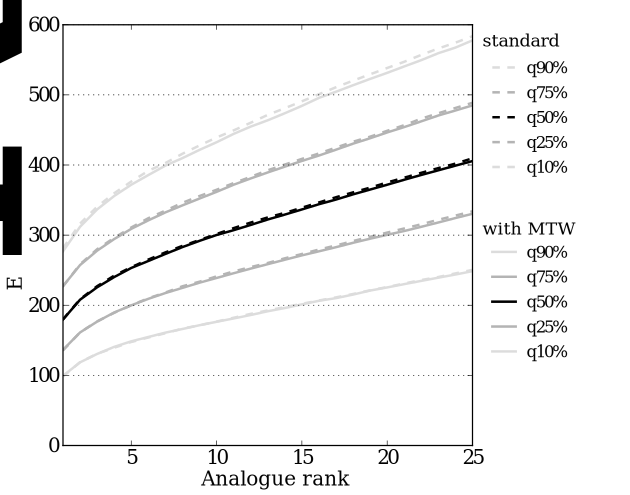
\includegraphics[width=8.1cm]{figures/changes_RMSE_value.pdf} \\
		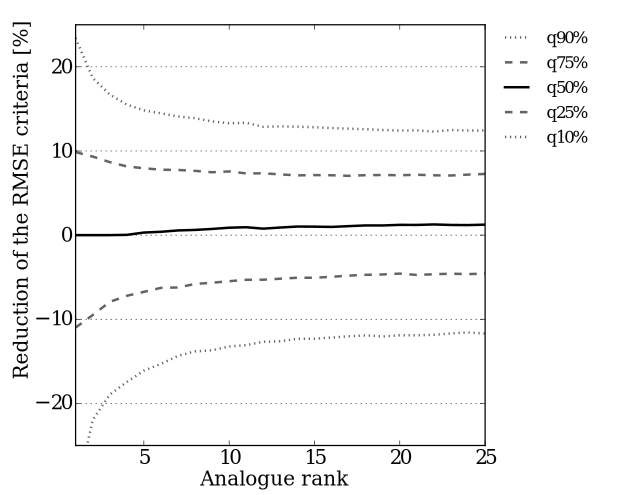
\includegraphics[width=8.3cm]{figures/changes_RMSE_gain.pdf}
	\end{center}
	\caption{Synthesis of the changes in the RMSE criteria, due to the STW, for the Ulrichen station, depending on the ranks of the analogue. (top) Quantiles of the RMSE distributions with and without the sliding window. (bottom) Quantiles of the relative improvements of the RMSE criteria when using the sliding window.}
	\label{fig:changes_RMSE}
\end{figure}

This result of a globally null improvement of the RMSE values does not mean that the 2Z-2MI method cannot be improved by the STW. It means that after the selection of the analogues situations in terms of the synoptic circulation, the new candidate dates do not allow to find better analogues in terms of moisture. However, the selected dates have changed in the first level of analogy, and thus also in the final selection, which can potentially improve the performance scores.


\section{Impact on performance scores}

A systematic improvement of the S1 values was previously observed. However, finding better analogue situations does not obligatory imply better forecast skills. Therefore, we have to assess the impact of the introduction of the sliding time window, and thus the selection of other analogue dates, on the performance scores. In order to perform this assessment, the 24~h-totals (moving average) at a 6-hourly time step were used (see section \ref{sec:data}). The target dates remain unchanged, since we keep the original time slot (6~h~UTC - 6~h~UTC the next day), and thus the performance scores can be directly compared with the former ones.

The new performance scores are provided in Table \ref{table:CRPSS_STW}, along with the differences regarding the conventional method with the same archive length. The differences ranges from 0.57 to 2.14 points for the 2Z method and from 1.53 to 2.20 points for the 2Z-2MI method. The introduction of the STW brings an improvement of the performance that is not very large, but that is nevertheless significant. Moreover, it requires no additional predictor. No relationship was found between the improvement of the score and the reduction of the S1 criteria, neither with the season.

\begin{table}[htb]
	\caption{New CRPSS performance scores for both 2Z and 2Z-2MI methods obtained by the STW approach. The differences are expressed regarding the conventional method with the same archive length.}
	\begin{center}
		\begin{tabular}{l c c c c}
			\hline
			\multirow{2}{*}{Station} & \multicolumn{2}{c}{2Z} & \multicolumn{ 2}{c}{2Z-2MI} \\
			& STW & $\Delta$ & STW & $\Delta$ \\
			\hline
			Ulrichen & 31.12 & 1.74 & 35.44 & 2.20 \\
			Zermatt & 24.34 & 2.14 & 28.92 & 1.97 \\
			Visp & 24.39 & 1.16 & 29.42 & 1.64 \\
			Montana & 31.59 & 0.80 & 36.30 & 1.53 \\
			Sion & 25.35 & 0.57 & 31.07 & 1.71 \\
			Aigle & 31.78 & 1.21 & 38.11 & 2.16 \\ 
			\hline
		\end{tabular}
	\end{center}
	\label{table:CRPSS_STW}
\end{table}


\subsection{Improvement by precipitation threshold}
\label{sec:improvement_CRPSS_precip_threshold}

The S1 criteria was previously found to be improved to a greater extent for the most dynamic situations related with higher precipitation values (section \ref{sec:influence_precip}). The changes in terms of performance scores will now be assessed regarding precipitation thresholds. Figure \ref{fig:changes_CRPS_precip_threshold} synthesizes these differences for the Ulrichen station, other stations having the same behavior.

The increasing positive trend of skill improvements regarding the precipitation threshold is significant and shows that the prediction of higher precipitation totals is further improved. Thus both the analogy criteria and the performance scores are improved to a greater extent for heavier precipitation events. On the contrary, the non-rainy days and small accumulations are not improved.

\begin{figure}[htb]
	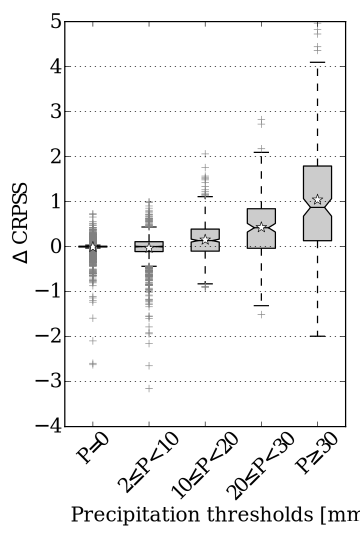
\includegraphics[width=5cm]{figures/changes_CRPS_precip_threshold.pdf}
	\caption{Differences of the CRPSS performance score, due to the introduction of the sliding time window, as a function of precipitation thresholds at the Ulrichen station. The stars represent averages.}
	\label{fig:changes_CRPS_precip_threshold}
\end{figure}


\subsection{Recalibrating the parameters}
\label{sec:recalibration}

The previous assessment of the performance improvement was established with the original parameters. However, one can assume that the introduction of the STW may change the optimum of some parameters. The calibration has then been performed again.

\begin{table}[htb]
	\caption{Calibrated parameters (spatial windows and number of analogues) for the analogy on the geopotential at 500~hPa and 1000~hPa (method 2Z) with the STW approach.}
	\begin{center}
		\begin{tabular}{l c c c }
			\hline
			Station & Longitudes & Latitudes & N$_{1}$ \\
			\hline
			Ulrichen & 0 $\rightarrow$ 17.5 & 42.5 $\rightarrow$ 50 & 50 \\
			Zermatt & 0 $\rightarrow$ 17.5 & 40 $\rightarrow$ 50 & 55 \\
			Visp & -2.5 $\rightarrow$ 20 & 40 $\rightarrow$ 50 & 55 \\
			Montana & -2.5 $\rightarrow$ 15 & 42.5 $\rightarrow$ 47.5 & 55 \\
			Sion & -2.5 $\rightarrow$ 15 & 37.5 $\rightarrow$ 50 & 55 \\
			Aigle & -2.5 $\rightarrow$ 15 & 40 $\rightarrow$ 50 & 75 \\
			\hline
		\end{tabular}
	\end{center}
	\label{table:params_2Z_new}
\end{table}

\begin{table}[htb]
	\caption{Parameters of the moisture variables from the 2Z-2MI method with the STW approach. The parameters for the atmospheric circulation are the same as in Table \ref{table:params_2Z_new}, except the number of analogues of the first analogy level (N$_{1}$), which are here different. The $5^{th}$ column is the number of analogues for the second level (N$_{2}$).}
	\begin{center}
		\begin{tabular}{l c c c c }
			\hline
			Station & Longitudes & Latitudes & N$_{1}$ & N$_{2}$ \\
			\hline
			Ulrichen & 5 $\rightarrow$ 10 & 45 $\rightarrow$ 47.5 & 110 & 35 \\
			Zermatt & 7.5 & 45 $\rightarrow$ 47.5 & 80 & 30 \\
			Visp & 7.5 & 45 $\rightarrow$ 47.5 & 135 & 35 \\
			Montana & 5 $\rightarrow$ 7.5 & 45 & 110 & 40 \\
			Sion & 5 $\rightarrow$ 10 & 45 $\rightarrow$ 47.5 & 140 & 50 \\
			Aigle & 5 $\rightarrow$ 7.5 & 45 & 135 & 45 \\ 
			\hline
		\end{tabular}
	\end{center}
	\label{table:params_2Z-2MI_new}
\end{table}

After recalibrating, some changes in the optimal parameters can be observed for both 2Z (Table \ref{table:params_2Z_new}) and 2Z-2MI methods (Table \ref{table:params_2Z-2MI_new}). Among these, the east-west dimension of the spatial windows of the circulation analogy tends to decrease. More significantly, the optimal number of analogues increases after introducing the STW, of a significant order of magnitude: 25~\% to 83~\% for the 2Z method and 20~\% 67~\% for the 2Z-2MI method. The number of analogues of the first analogy level of the 2Z-2MI method even reached three times its previous value for the Visp station. As we saw in Figure \ref{fig:changes_S1}, the improvement of the S1 criteria grows along with the rank of the analogue, which shows an accumulation of better analogue situations in the distributions. It seems thus profitable to widen the selection of analogues in order to keep also some whose rank has increased, as they appear to be also relevant to predict precipitation values. The number of good analogues is thus globally increased.

This increase in number of analogues has a slight effect on the performance of the different precipitation classes. The same analysis as in section \ref{sec:improvement_CRPSS_precip_threshold} has been performed again on the basis of the newly calibrated parameters. The results are generally very similar, but a slight performance increase of small precipitation values can be observed at the expense of higher amounts. The change in the analogues numbers is likely to be responsible for this difference in the performance distributions.

\begin{table}[htb]
	\caption{Values of the CRPSS (\%) skill score for the newly calibrated parameters using the STW approach. The differences are expressed regarding the conventional method with the same archive length.}
	\begin{center}
		\begin{tabular}{l c c c c}
			\hline
			\multirow{2}{*}{Station} & \multicolumn{2}{c}{2Z} & \multicolumn{ 2}{c}{2Z-2MI} \\
			& STW & $\Delta$ & STW & $\Delta$ \\
			\hline
			Ulrichen & 31.58 & 2.20 & 35.72 & 2.48  \\
			Zermatt & 24.71 & 2.51 & 29.63 & 2.68 \\
			Visp & 25.08 & 1.85 & 30.29 & 2.52 \\
			Montana & 32.22 & 1.43 & 37.15 & 2.38 \\
			Sion & 26.07 & 1.29 & 31.68 & 2.32 \\
			Aigle & 32.21 & 1.64 & 38.50 & 2.55 \\
			\hline
		\end{tabular}
	\end{center}
	\label{table:CRPSS_recalibration}
\end{table}

The values of the CRPSS scores for both methods (Table \ref{table:CRPSS_recalibration}) have significantly increased after recalibration. With the introduction of the sliding time window, we get back the performance loss related to the reduction of the archive length. In our case, this improvement is approximately a doubling of the archive size.


\subsection{Changes in sharpness and accuracy}

The CRPS score can be decomposed into two components, namely sharpness and accuracy. The impact of the STW has been analyzed on these components and the results can be found in Table \ref{table:CRPSS_decomposition_no_recalibration} for the original parameters and in Table \ref{table:CRPSS_decomposition_recalibration} for the re-calibrated methods. The changes are expressed relative to the total CRPS. Both components do not have the same value ranges: accuracy is in our case almost twice the sharpness values. Since the CRPS is considered here and not the CRPSS, improved prediction capacity results in a lower score. A decrease of the score is thus desirable.

\begin{table}[htb]
	\caption{Changes in sharpness and accuracy relatively to the total CRPS, due to the introduction of the sliding time window. The changes are presented for both 2Z and 2Z-2MI methods with the original parameters. A decrease of the score is desirable.}
	\begin{center}
		\begin{tabular}{l c c c c}
			\hline
			\multirow{2}{*}{Station} & \multicolumn{2}{c}{2Z} & \multicolumn{2}{c}{2Z-2MI} \\
			& Sharpness & Accuracy & Sharpness & Accuracy \\
			\hline
			Ulrichen & 2.82 & -5.29 & 1.00 & -4.30 \\
			Zermatt & 2.26 & -5.01 & 0.88 & -3.58 \\
			Visp & 3.66 & -5.18 & 2.67 & -4.94 \\
			Montana & 1.62 & -2.78 & 0.57 & -2.91 \\
			Sion & 2.02 & -2.78 & 0.33 & -2.75 \\
			Aigle & 0.52 & -2.26 & -1.20 & -2.17 \\ 
			\hline
		\end{tabular}
	\end{center}
	\label{table:CRPSS_decomposition_no_recalibration}
\end{table}


\begin{table}[htb]
	\caption{Same as Table \ref{table:CRPSS_decomposition_no_recalibration} but with the re-calibrated parameters.}
	\begin{center}
		\begin{tabular}{l c c c c}
			\hline
			\multirow{2}{*}{Station} & \multicolumn{2}{c}{2Z} & \multicolumn{2}{c}{2Z-2MI} \\
			& Sharpness & Accuracy & Sharpness & Accuracy \\
			\hline
			Ulrichen & 1.44 & -4.56 & -0.37 & -3.34 \\
			Zermatt & 0.80 & -4.03 & 0.75 & -4.42 \\
			Visp & 1.53 & -3.94 & 1.47 & -4.96 \\
			Montana & -0.27 & -1.80 & 0.06 & -3.71 \\
			Sion & 0.95 & -2.66 & -0.10 & -3.19 \\
			Aigle & -0.35 & -2.01 & -2.08 & -1.90 \\ 
			\hline
		\end{tabular}
	\end{center}
	\label{table:CRPSS_decomposition_recalibration}
\end{table}

\begin{figure*}[htb]
	\begin{center}$
		\begin{array}{cccc}
		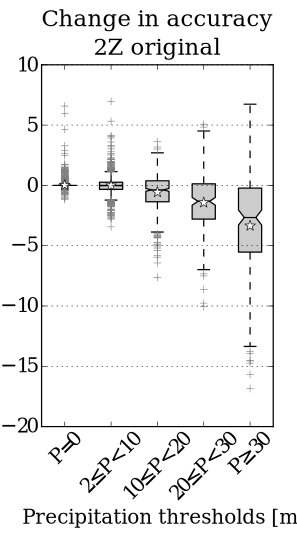
\includegraphics[width=4cm]{figures/component_2Z_accuracy.pdf} &
		\includegraphics[width=4cm]{figures/component_2Z_sharpness.pdf} &
		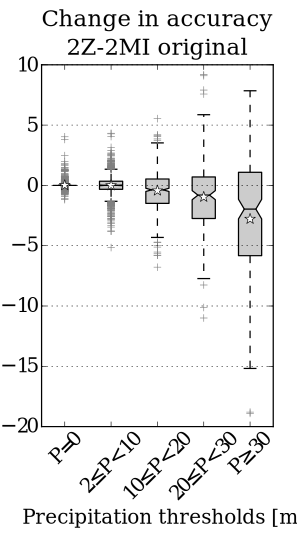
\includegraphics[width=4cm]{figures/component_2Z-2MI_accuracy.pdf} &
		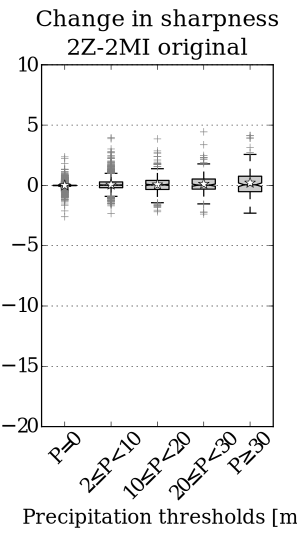
\includegraphics[width=4cm]{figures/component_2Z-2MI_sharpness.pdf} \\ \\
		\includegraphics[width=4cm]{figures/component_2Z_accuracy_recalib.pdf} &
		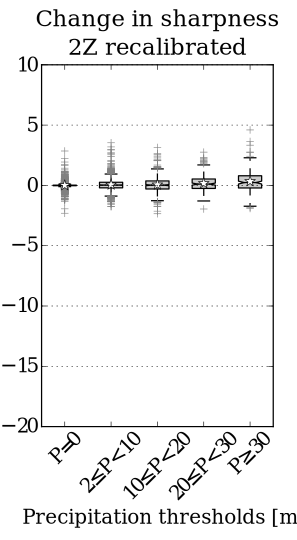
\includegraphics[width=4cm]{figures/component_2Z_sharpness_recalib.pdf} &
		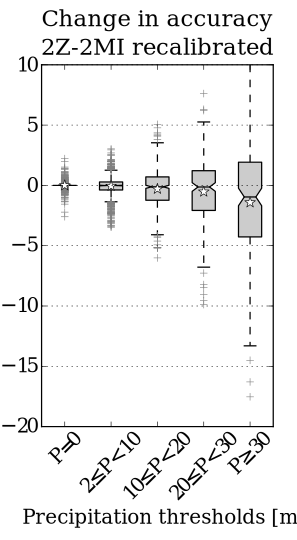
\includegraphics[width=4cm]{figures/component_2Z-2MI_accuracy_recalib.pdf} &
		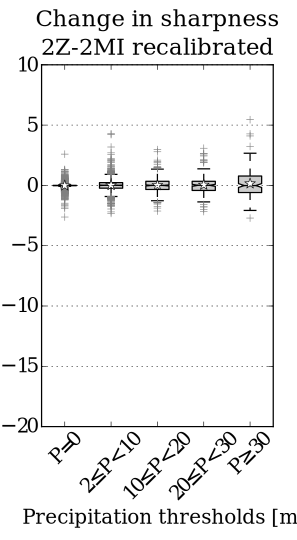
\includegraphics[width=4cm]{figures/component_2Z-2MI_sharpness_recalib.pdf} 
		\end{array}$
	\end{center}
	\caption{Influence (\%) of the STW on the CRPS components (accuracy and sharpness) relatively to the total CRPS, for the 2Z and 2Z-2MI methods, according to different precipitation thresholds. The results are presented for (top) the original parameters, and (bottom) the recalibrated parameters. Improved prediction results in a lower score.}
	\label{fig:CRPSS_decomposition_precip_thresholds}
\end{figure*}

It appears that the sharpness is a bit inferior with the STW in favor of accuracy (Table \ref{table:CRPSS_decomposition_no_recalibration}). When using the recalibrated parameters, the components are a bit more balanced, but still the accuracy prevails on the sharpness (Table \ref{table:CRPSS_decomposition_recalibration}). Figure \ref{fig:CRPSS_decomposition_precip_thresholds} illustrates the changes (relative to the total CRPS) in sharpness and accuracy for different precipitation thresholds at the Ulrichen station. Be it for the 2Z or 2Z-2MI method, the original or the recalibrated parameters, the changes are similar: the improvements concern the accuracy over the sharpness, and this to a greater extent for significant precipitation events. The STW does not allow to improve the sharpness, but the improvement in accuracy is significant, and this especially for the days with heavy precipitation. In terms of the predicted precipitation distribution, it means that the median of the prediction is closer to the observed values, but the distribution is not more condensed than previously.


\section{Application attempts on the full archive}

The improvement provided by the STW is interesting, mainly for heavy precipitation events, and thus it would be profitable to be able to apply it to the complete archive. Unfortunately, there is no long precipitation time series available with a sub-daily time step. In order to reconstruct a longer archive of moving averages of 24~h-totals, different disaggregation approaches of the daily time series were assessed and are presented in the following sections.

\subsection{Proportional distribution}

A proportional distribution is certainly the simplest approach that can be performed. It consists in allocating proportional parts of the original daily time series into a new moving average of 24~h-totals (Figure \ref{fig:illustration_disaggregation}). When using this reconstructed time series on the shorter period, the method performance was degraded (Table \ref{table:disaggregation_proportional} to compare to Table \ref{table:CRPSS_STW}) and was even below the conventional method without STW (Table \ref{table:loss_reduction}). The benefit of a better selection of the analogue situations is lost due to a precipitation archive of poor quality.

\begin{figure}[htb]
	\begin{center}
		\includegraphics[width=8cm]{figures/illustration_disaggregation.pdf}
	\end{center}
	\caption{Illustration of the generation of 24~h-totals moving averages by means of a proportional distribution.}
	\label{fig:illustration_disaggregation}
\end{figure}

\begin{table}[htb]
	\caption{Values of the CRPSS (\%) skill score for the original and the recalibrated parameters using the STW approach on the disaggregated precipitation time series (short period) by means of the proportional distribution.}
	\begin{center}
		\begin{tabular}{l c c c c}
			\hline
			\multirow{2}{*}{Station} & \multicolumn{2}{c}{2Z} & \multicolumn{ 2}{c}{2Z-2MI} \\
			& original & recalib. & original & recalib. \\
			\hline
			Ulrichen & 29.13 & 29.61 & 33.15 & 33.45 \\
			Zermatt & 22.17 & 22.80 & 26.72 & 27.43 \\
			Visp & 22.32 & 22.89 & 27.01 & 28.04 \\
			Montana & 29.41 & 30.24 & 33.83 & 34.55 \\
			Sion & 22.98 & 23.41 & 28.57 & 29.15 \\
			Aigle & 29.07 & 29.46 & 34.66 & 35.09 \\
			\hline
		\end{tabular}
	\end{center}
	\label{table:disaggregation_proportional}
\end{table}



\subsection{Utilisation d'un proxy pour reconstituer la chronologie}

Comme nous l'avons vu dans la section précédente, une série de précipitations reconstituée de manière simpliste nous fait perdre tout le gain de performance de la fenêtre temporelle glissante et ne présente alors aucun intérêt. Nous devons donc trouver un moyen de nous approcher de la chronologie réelle, pour une période (1961-1981) où nous ne disposons d'aucune série de précipitations continue avec une résolution plus fine. Il nous faut donc extraire de l'information de la répartition intrajournalière des pluies à partir d'une autre source de données. Un modèle de prévision météorologique régional serait en mesure d'apporter de l'information permettant de générer des séries de précipitations plus pertinentes. Malheureusement, de tels résultats ne sont pas disponibles sous forme de longues archives. Une alternative aux modèles régionaux est donnée par les réanalyses. Bien que celles-ci ont une résolution plus faible et n'intègrent que grossièrement les processus locaux, nous allons évaluer si elles rendent possible la transposition de la fenêtre temporelle glissante sur toute l'archive. 

La première étape consiste à déterminer quelle variable, de l'eau précipitable ou de l'humidité relative, est la plus corrélée avec la série de précipitations sur la période 1982-2007, et en quel point. Nous considérons les niveaux 1000~hPa, 925~hPa et 850~hPa pour l'humidité relative, et les points les plus proches du bassin (5\textdegree\ - 7.5\textdegree\ de longitude et 45\textdegree\ - 47.5\textdegree\ de latitude). Finalement, les points de grille des réanalyses étant relativement éloignés de nos stations, il est pertinent de rechercher la présence probable d'un décalage temporel entre les séries. 

Le point le plus pertinent ne sera probablement pas le même pour toutes les stations, puisque nous pouvons nous attendre à trouver l'optimum dans la direction des apports d'humidité principaux pour la station. Cette recherche doit donc être effectuée pour chacune de nos stations. Nous illustrons le principe avec la station de Zermatt.


\begin{table}[htb]
	\caption{Valeur du coefficient de détermination entre les séries reconstituées à l'aide d'un proxy et la série réelle à pas de temps de 6~h. Les proxys évalués sont l'eau précipitable et l'humidité relative à différents niveaux atmosphériques, en 4 points proches du bassin. Le coefficient de détermination le plus élevé est indiqué en gras.}
	\begin{center}
		\begin{tabular}{|l|rr|rrrrr|}
			\cline{ 2- 8}
			\multicolumn{1}{l}{} & \multicolumn{2}{|c|}{\textbf{Position}} &  \multicolumn{5}{c|}{\textbf{Décalage temporel}} \\
			\multicolumn{1}{l}{} & \multicolumn{1}{|c}{\textbf{Lon}} & \multicolumn{1}{c|}{\textbf{Lat}} & \multicolumn{1}{c}{\textbf{-12h}} & \multicolumn{1}{c}{\textbf{-6h}} & \multicolumn{1}{c}{\textbf{0h}} & \multicolumn{1}{c}{\textbf{+6h}} & \multicolumn{1}{c|}{\textbf{+12h}} \\ \hline
			\multirow{ 4}{*}{RHum 1000 hPa} & 5.0 & 47.5 & 0.668 & 0.669 & 0.684 & 0.683 & 0.670 \\
			& 5.0 & 45.0 & 0.669 & 0.669 & 0.683 & 0.681 & 0.669 \\
			& 7.5 & 47.5 & 0.662 & 0.673 & 0.691 & 0.682 & 0.673 \\
			& 7.5 & 45.0 & 0.666 & 0.671 & 0.688 & 0.681 & 0.668 \\ \hline
			\multirow{ 4}{*}{RHum 925 hPa} & 5.0 & 47.5 & 0.672 & 0.673 & 0.684 & 0.684 & 0.675 \\
			& 5.0 & 45.0 & 0.674 & 0.674 & 0.683 & 0.682 & 0.672 \\
			& 7.5 & 47.5 & 0.662 & 0.673 & 0.691 & 0.682 & 0.673 \\
			& 7.5 & 45.0 & 0.666 & 0.671 & 0.689 & 0.681 & 0.668 \\ \hline
			\multirow{ 4}{*}{RHum 850 hPa} & 5.0 & 47.5 & 0.675 & 0.675 & 0.679 & 0.678 & 0.671 \\
			& 5.0 & 45.0 & 0.681 & 0.690 & 0.691 & 0.677 & 0.664 \\
			& 7.5 & 47.5 & 0.665 & 0.680 & 0.693 & 0.683 & 0.675 \\
			& 7.5 & 45.0 & 0.675 & 0.694 & 0.706 & 0.681 & 0.659 \\ \hline
			\multirow{ 4}{*}{Eau precipitable} & 5.0 & 47.5 & 0.688 & 0.687 & 0.667 & 0.655 & 0.652 \\
			& 5.0 & 45.0 & 0.697 & 0.699 & 0.669 & 0.644 & 0.644 \\
			& 7.5 & 47.5 & 0.686 & 0.708 & 0.689 & 0.655 & 0.648 \\
			& 7.5 & 45.0 & 0.696 & \textbf{0.721} & 0.696 & 0.643 & 0.636 \\ \hline
		\end{tabular}
	\end{center}
	\label{tab:fenetre_glissante:Serie_proxy_correlations}
\end{table}

\begin{table}[htb]
	\caption{Valeurs des scores CRPSS pour Zermatt avec la série glissée reconstituée à l'aide d'un proxy météorologique. Les résultats sont présentés pour les deux périodes 1982-2007 et 1961-2008, pour les paramètres sans et avec recalibration, ainsi que pour les deux méthodes R1 et R2.}
	\begin{center}
		\begin{tabular*}{10cm}{@{\extracolsep{\fill}}lcccc}
			\hline
			\multirow{2}{*}{\textbf{Période}} & \multicolumn{ 2}{c}{\textbf{Sans recalibration}} & \multicolumn{ 2}{c}{\textbf{Avec recalibration}} \\
			& \multicolumn{1}{c}{\textbf{R1}} & \textbf{R2} & \multicolumn{1}{c}{\textbf{R1}} & \textbf{R2} \\ \hline
			1982-2007 & 22.57~\% & 27.11~\% & 23.14~\% & 27.71~\% \\ \hline
			1961-2008 & 23.81~\% & 28.42~\% & 24.38~\% & 28.86~\% \\ \hline
		\end{tabular*}
	\end{center}
	\label{tab:fenetre_glissante:Resultats_proxy_Zermatt}
\end{table}


Afin de déterminer quelle variable météorologique considérer, en quel point, et avec quel décalage horaire, chacune des séries générées doit être comparée à la série réelle. La Table \ref{tab:fenetre_glissante:Serie_proxy_correlations} présente les coefficients de détermination sur les valeurs non nulles entre les nouvelles séries reconstituées à l'aide du proxy et la série réelle de la station de Zermatt à pas de temps de 6~h sur la période 1982-2007. Le meilleur proxy est l'eau précipitable à 45\textdegree\ de latitude et 7.5\textdegree\ de longitude, avec un décalage temporel de -6~h; cela signifie que nous devons retarder de 6~h la chronologie du prédicteur afin de l'appliquer aux précipitations. Le coefficient de détermination de 0.721 est supérieur à celui de la série par moyenne mobile (0.698), ce qui nous confirme que nous avons ajouté un peu d'information à la série de précipitations, sans toutefois savoir si celle-ci est suffisante.

La Table \ref{tab:fenetre_glissante:Resultats_proxy_Zermatt} présente les scores CRPSS obtenus par la série reconstituée à l'aide du proxy de l'eau précipitable au point optimal (Table \ref{tab:fenetre_glissante:Serie_proxy_correlations}). Nous observons une légère amélioration par rapport aux résultats obtenus avec la série de moyennes mobiles (Table \ref{tab:fenetre_glissante:Resultats_moyenne_mobile}), mais celle-ci est toujours relativement petite, et la plus grande partie du gain de la fenêtre temporelle glissante est perdue.

Ces tentatives de transposition de la fenêtre temporelle glissante sur l'archive totale mettent en évidence l'importance de la temporalité réelle des précipitations. La fenêtre glissante est un gain, à condition que les séries de précipitations soient proches de l'observé. Sans information sur la chronologie des précipitations, il n'est pas pertinent d'appliquer cette modification à la méthode. Nous pouvons espérer que, dans le futur, des reprévisions par des modèles régionaux seront en mesure de nous apporter une chronologie des précipitations s'approchant de la réalité.


\conclusions  %% \conclusions[modified heading if necessary]

Comme \citet{Finet2008} l'avaient déjà été montré précédemment, nous gagnons en analogie synoptique en introduisant la fenêtre temporelle glissante. Pour ce qui est de la prévision des précipitations, nous regagnons en fenêtre glissante sur période réduite ce que nous avions perdu par rapport à la fenêtre fixe en raison de la réduction de l'archive. Dans notre cas, ce gain correspond au doublement de la taille de l'archive.

Nous avons également démontré l'importance de la qualité de l'archive pluviométrique: nous gagnons en prévision des précipitations pour autant que la chronologie des pluies y soit proche de la réalité. Pour une archive reconstituée de manière grossière, les gains en performances de la fenêtre glissante ne se répercutent pas sur la prévision des pluies, bien que l'analogie synoptique soit meilleure. Il conviendra donc de maintenir l'objectif qui consiste à reconstruire des séries de précipitations passées de manière la plus réaliste possible, par exemple à l'aide d'un modèle météorologique régional. Lorsque de telles archives pluviométriques seront disponibles, l'ajout d'une fenêtre temporelle glissante en prévision par analogie montrera tout son intérêt.




\appendix
\section{}    %% Appendix A

\subsection{}                               %% Appendix A1, A2, etc.




\begin{acknowledgements}
Thanks to Dominique B\'{e}rod for his support and to Renaud Marty for his fruitful collaboration over the years. Thanks to the Swiss Federal Office for Environment (FOEV), the Roads and Water courses Service, Energy and Water Power Service of the Wallis Canton and the Water, Land and Sanitation Service of the Vaud Canton who financed the MINERVE (Mod\'{e}lisation des Intemp\'{e}ries de Nature Extr\^{e}me des Rivi\`{e}res Valaisannes et de leurs Effets) project which started this research. The fruitful collaboration with the Laboratoire d'Etude des Transferts en Hydrologie et Environnement of the Grenoble Institute of Technology (G-INP) was made possible thanks to the Herbette Foundation. NCEP reanalysis data provided by the NOAA/OAR/ESRL PSD, Boulder, Colorado, USA, from their Web site at http://www.esrl.noaa.gov/psd/. Precipitation time series provided by MeteoSwiss. 
\end{acknowledgements}


%% REFERENCES

%% The reference list is compiled as follows:

\bibliographystyle{copernicus}
\bibliography{../_refs/_articles-moving-window}

%% Since the Copernicus LaTeX package includes the BibTeX style file copernicus.bst,
%% authors experienced with BibTeX only have to include the following two lines:
%%
%% \bibliographystyle{copernicus}
%% \bibliography{example.bib}
%%
%% URLs and DOIs can be entered in your BibTeX file as:
%%
%% URL = {http://www.xyz.org/~jones/idx_g.htm}
%% DOI = {10.5194/xyz}


%% LITERATURE CITATIONS
%%
%% command                        & example result
%% \citet{jones90}|               & Jones et al. (1990)
%% \citep{jones90}|               & (Jones et al., 1990)
%% \citep{jones90,jones93}|       & (Jones et al., 1990, 1993)
%% \citep[p.~32]{jones90}|        & (Jones et al., 1990, p.~32)
%% \citep[e.g.,][]{jones90}|      & (e.g., Jones et al., 1990)
%% \citep[e.g.,][p.~32]{jones90}| & (e.g., Jones et al., 1990, p.~32)
%% \citeauthor{jones90}|          & Jones et al.
%% \citeyear{jones90}|            & 1990



%% FIGURES

%% ONE-COLUMN FIGURES

%%f
%\begin{figure}[t]
%\includegraphics[width=8.3cm]{FILE NAME}
%\caption{TEXT}
%\end{figure}
%
%%% TWO-COLUMN FIGURES
%
%%f
%\begin{figure*}[t]
%\includegraphics[width=12cm]{FILE NAME}
%\caption{TEXT}
%\end{figure*}
%
%
%%% TABLES
%%%
%%% The different columns must be seperated with a & command and should
%%% end with \\ to identify the column brake.
%
%%% ONE-COLUMN TABLE
%
%%t
%\begin{table}[t]
%\caption{TEXT}
%\begin{tabular}{column = lcr}
%\tophline
%
%\middlehline
%
%\bottomhline
%\end{tabular}
%\belowtable{} % Table Footnotes
%\end{table}
%
%%% TWO-COLUMN TABLE
%
%%t
%\begin{table*}[t]
%\caption{TEXT}
%\begin{tabular}{column = lcr}
%\tophline
%
%\middlehline
%
%\bottomhline
%\end{tabular}
%\belowtable{} % Table Footnotes
%\end{table*}
%
%
%%% NUMBERING OF FIGURES AND TABLES
%%%
%%% If figures and tables must be numbered 1a, 1b, etc. the following command
%%% should be inserted before the begin{} command.
%
%\addtocounter{figure}{-1}\renewcommand{\thefigure}{\arabic{figure}a}
%
%
%%% MATHEMATICAL EXPRESSIONS
%
%%% All papers typeset by Copernicus Publications follow the math typesetting regulations
%%% given by the IUPAC Green Book (IUPAC: Quantities, Units and Symbols in Physical Chemistry,
%%% 2nd Edn., Blackwell Science, available at: http://old.iupac.org/publications/books/gbook/green_book_2ed.pdf, 1993).
%%%
%%% Physical quantities/variables are typeset in italic font (t for time, T for Temperature)
%%% Indices which are not defined are typeset in italic font (x, y, z, a, b, c)
%%% Items/objects which are defined are typeset in roman font (Car A, Car B)
%%% Descriptions/specifications which are defined by itself are typeset in roman font (abs, rel, ref, tot, net, ice)
%%% Abbreviations from 2 letters are typeset in roman font (RH, LAI)
%%% Vectors are identified in bold italic font using \vec{x}
%%% Matrices are identified in bold roman font
%%% Multiplication signs are typeset using the LaTeX commands \times (for vector products, grids, and exponential notations) or \cdot
%%% The character * should not be applied as mutliplication sign
%
%
%%% EQUATIONS
%
%%% Single-row equation
%
%\begin{equation}
%
%\end{equation}
%
%%% Multiline equation
%
%\begin{align}
%& 3 + 5 = 8\\
%& 3 + 5 = 8\\
%& 3 + 5 = 8
%\end{align}
%
%
%%% MATRICES
%
%\begin{matrix}
%x & y & z\\
%x & y & z\\
%x & y & z\\
%\end{matrix}
%
%
%%% ALGORITHM
%
%\begin{algorithm}
%\caption{…}
%\label{a1}
%\begin{algorithmic}
%…
%\end{algorithmic}
%\end{algorithm}
%
%
%%% CHEMICAL FORMULAS AND REACTIONS
%
%%% For formulas embedded in the text, please use \chem{}
%
%%% The reaction environment creates labels including the letter R, i.e. (R1), (R2), etc.
%
%\begin{reaction}
%%% \rightarrow should be used for normal (one-way) chemical reactions
%%% \rightleftharpoons should be used for equilibria
%%% \leftrightarrow should be used for resonance structures
%\end{reaction}
%
%
%%% PHYSICAL UNITS
%%%
%%% Please use \unit{} and apply the exponential notation


\end{document}
